\documentclass[conference]{IEEEtran}
\usepackage{cite}
\usepackage{amsmath,amssymb}
\usepackage{graphicx}
\usepackage{booktabs}
\usepackage{tikz}
\usetikzlibrary{arrows.meta,positioning}
\usepackage{url}
\usepackage[hidelinks]{hyperref}
\graphicspath{{figures/}}
\hypersetup{
  pdftitle={Automated Memory Forensics for Malware Detection and Incident Response},
  pdfauthor={Joel C. Okore, Andrei Petrovski, Igor V. Kotenko},
  pdfkeywords={memory forensics, incident response, security automation, malware detection}
}

\begin{document}

\title{Automated Memory Forensics for\\
Malware Detection and Incident Response}

\author{\IEEEauthorblockN{Joel C. Okore}
\IEEEauthorblockA{\textit{Faculty of Computer Science} \\
\textit{Innopolis University}\\
Innopolis, Tatarstan, Russia \\
j.okore@innopolis.university}
\and
\IEEEauthorblockN{Andrei Petrovski}
\IEEEauthorblockA{\textit{Faculty of Computer Science} \\
\textit{Innopolis University}\\
Innopolis, Tatarstan, Russia \\
a.petrovski@innopolis.ru}
\and
\IEEEauthorblockN{Igor V. Kotenko}
\IEEEauthorblockA{\textit{Security Problems Lab} \\
\textit{SPC RAS}\\
St. Petersburg, Russia \\
ivkote@comsec.spb.ru}
\IEEEauthorblockA{\textit{Institute of Information Security} \\
\textit{Innopolis University}\\
Innopolis, Tatarstan, Russia \\
i.kotenko@innopolis.ru}}

\maketitle

\begin{abstract}
Memory forensics can provide evidence of malicious activity that is unavailable from endpoint alerts alone, but acquisition, analysis, and response often require separate operational steps. This paper presents an automated memory-forensics pipeline that connects these steps through an event-driven workflow. Wazuh alerts trigger remote memory acquisition using WinPMEM; file-integrity events initiate Volatility3 for memory analysis and extraction of forensic artifacts, which will then be used as features for machine learning classification; and a malicious prediction invokes network isolation and an analyst notification. The implementation uses a Windows endpoint, an Ubuntu manager, and explicit file and message interfaces between the stages of the pipeline. The case study in consideration demonstrates the workflow from an endpoint alert through memory acquisition, classification, and automated response. In the isolated experiment, WannaCry ransomware was detonated on a monitored endpoint, the pipeline was triggered automatically and progressed from memory acquisition to response initiation in under three minutes. Execution logs and a subsequent connectivity test document the observed response behavior. Supporting experiments examine classifier portability and a host-relative scoring extension, identifying requirements for calibration and clean-reference integrity. The main contribution is the design, implementation and integration of the forensic response workflow, together with the operational lessons needed to extend it.
\end{abstract}

\begin{IEEEkeywords}
memory forensics, incident response, security automation, malware detection, Wazuh, Volatility3
\end{IEEEkeywords}

\section{Introduction}

Security operations depend on both detecting suspicious activity and obtaining the evidence needed to investigate it. Endpoint logs can indicate an unusual command or process, while a memory image provides a basis for examining the system state associated with that activity. Because volatile artifacts can disappear when processes terminate or memory is reused, initiating acquisition is an operational concern.

A practical memory forensics workflow must coordinate several tools. An alert must identify the endpoint, a privileged acquisition utility must obtain its memory image, the image must become accessible to an analysis host, and the analysis result must reach a response mechanism. When these transitions require manual intervention, an analyst must repeatedly transfer context between detection, forensic analysis, and containment. Automating the transitions provides a way to connect forensic collection to an existing incident response workflow.

In this work, we design and implement such a workflow using Wazuh active response~\cite{wazuh}, WinPMEM~\cite{winpmem}, Volatility3~\cite{volatility}, and a machine learning classifier. Wazuh coordinates the workflow: endpoint alerts trigger memory acquisition, while file-integrity events initiate feature extraction from the captured image and classification of the resulting feature vector. The classifier returns a structured decision that the response script uses to request network isolation and notify the security team. The system therefore connects collection, analysis, and response action using interfaces available in an open-source security stack.

The application setting is a Windows endpoint monitored by an Ubuntu Wazuh manager. We evaluate functional integration through an isolated WannaCry case study, examining the artifacts and logs produced as the workflow executes. A supporting assessment of the classifier and a host-relative extension addresses what additional evidence is needed before transferring automated response to different hosts and workloads.

The contributions are:
\begin{enumerate}
\item An event-driven architecture that connects endpoint detection to remote memory acquisition, forensic feature extraction, and automated response. 
\item A working implementation with explicit artifact and message interfaces, demonstrated through a WannaCry ransomware case study with execution logs and observed connectivity loss after endpoint isolation action.
\item An assessment of deployment requirements, including stage completion, response verification, classifier portability, and baseline integrity.
\end{enumerate}

\section{Related Work}

% \subsection{Forensic Automation and System Integration}
Remote collection is an established approach to incorporating forensic
evidence into incident response. Cohen et al.~\cite{cohen2011} introduce
GRR Rapid Response as a distributed framework for enterprise investigations,
providing remote access to memory and raw disk data. Its client--server
architecture supports forensic tasks across multiple operating systems and
addresses the coordination required when evidence resides on remote endpoints.
GRR is discussed here as related work on distributed evidence collection; it
is not part of the implemented system, which instead uses Wazuh active
response and WinPMEM as described in Section~\ref{sec:architecture}.

SPECTRE, proposed by Syed et al.~\cite{syed2026}, integrates memory-snapshot
comparison, anomaly detection, network-artifact analysis, and visualization.
It uses Volatility JSON output as an intermediate representation and includes
emulated artifacts for controlled evaluation. This work illustrates how
structured forensic output can support several analysis components within
one system. It also provides a relevant point of comparison for the explicit
artifact and decision interfaces used in the present implementation.

The components used here provide the mechanisms for connecting such analysis
to endpoint actions. Wazuh active response associates scripts with detection
rules, severity levels, or rule groups~\cite{wazuh}. WinPMEM acquires physical
memory as a raw image~\cite{winpmem}, and Volatility3 extracts forensic
artifacts from that image~\cite{volatility}. Their integration requires a
defined sequence of triggers, artifact transfers, and response decisions,
which forms the systems focus of this paper.

% \subsection{Malware Classification and Analyst Support}
Machine learning based memory image classification automates part of the interpretation of
forensic artifacts. VolMemLyzer~\cite{lashkari2021} extracts memory features
for malware classification. Carrier et al.~\cite{carrier2022} evaluate this
approach on obfuscated malware in CIC-MalMem-2022, reporting 99.00\% accuracy
and a 99.02\% F1-score for a stacked ensemble. These studies establish
memory image classification as a candidate decision component, while its
operational use requires evaluation on the endpoints where decisions are
applied.

Okore et al.~\cite{okore2026} examine explainable malware detection from
encrypted network-traffic metadata. Their approach combines fast per-flow
explanations with on-demand analysis for analyst investigation, evaluating
detection performance alongside explanation latency and stability. The study
connects model interpretation to security operations. The present work
addresses a complementary requirement: collecting volatile endpoint evidence
after an alert and processing it through forensic analysis to a containment
decision. The two studies concern different evidence sources and different
parts of the incident-response process.

The reliability of the decision component remains relevant to either
application. Arp et al.~\cite{arp2022} identify sampling bias, data leakage,
and other evaluation pitfalls in security machine learning. These concerns
motivate the supporting classifier assessment in Section~\ref{sec:assessment}.
The contribution evaluated here is the integration of alert-driven memory
acquisition, forensic classification, and automated response in a working
Windows--Ubuntu deployment.

\section{System Design and Implementation}
\label{sec:architecture}

\subsection{Operational Objectives}
The system is designed around three objectives: initiate memory dump collection triggered by an endpoint alert, pass the resulting evidence through analysis without manual invocation, and connect the resulting decision of the analysis to endpoint containment and analyst notification. Memory acquisition precedes network isolation so that the manager can obtain and analyze the image while its management and data paths remain available. 
% This ordering makes acquisition part of the response workflow and also introduces a delay before containment.

The Windows 10 endpoint runs the Wazuh agent and WinPMEM. It is configured to supply PowerShell operational events and exposes the memory dump directory through an SMB-shared network folder. The Ubuntu manager hosts Wazuh rules, active-response scripts, Volatility3, the serialized classifier, and the notification client. Memory dump acquisition and endpoint isolation use Windows Remote Management (WinRM), invoked through NetExec. The image is made available to the manager through the SMB-shared network directory. Fig.~\ref{fig:architecture} shows the component placement and system architecture.

This placement keeps forensic parsing and model inference on the manager, while the endpoint provides event collection and memory acquisition. The analysis environment can therefore be maintained centrally, including the Volatility installation and the classifier's preprocessing bundle. Changes confined to these components do not require redeploying the endpoint acquisition utility. The shared directory forms the boundary between endpoint-specific collection and the manager's analysis environment.

The prototype implementation source code is available in the project repository~\cite{projectrepo}.

\begin{figure}[!t]
\centering
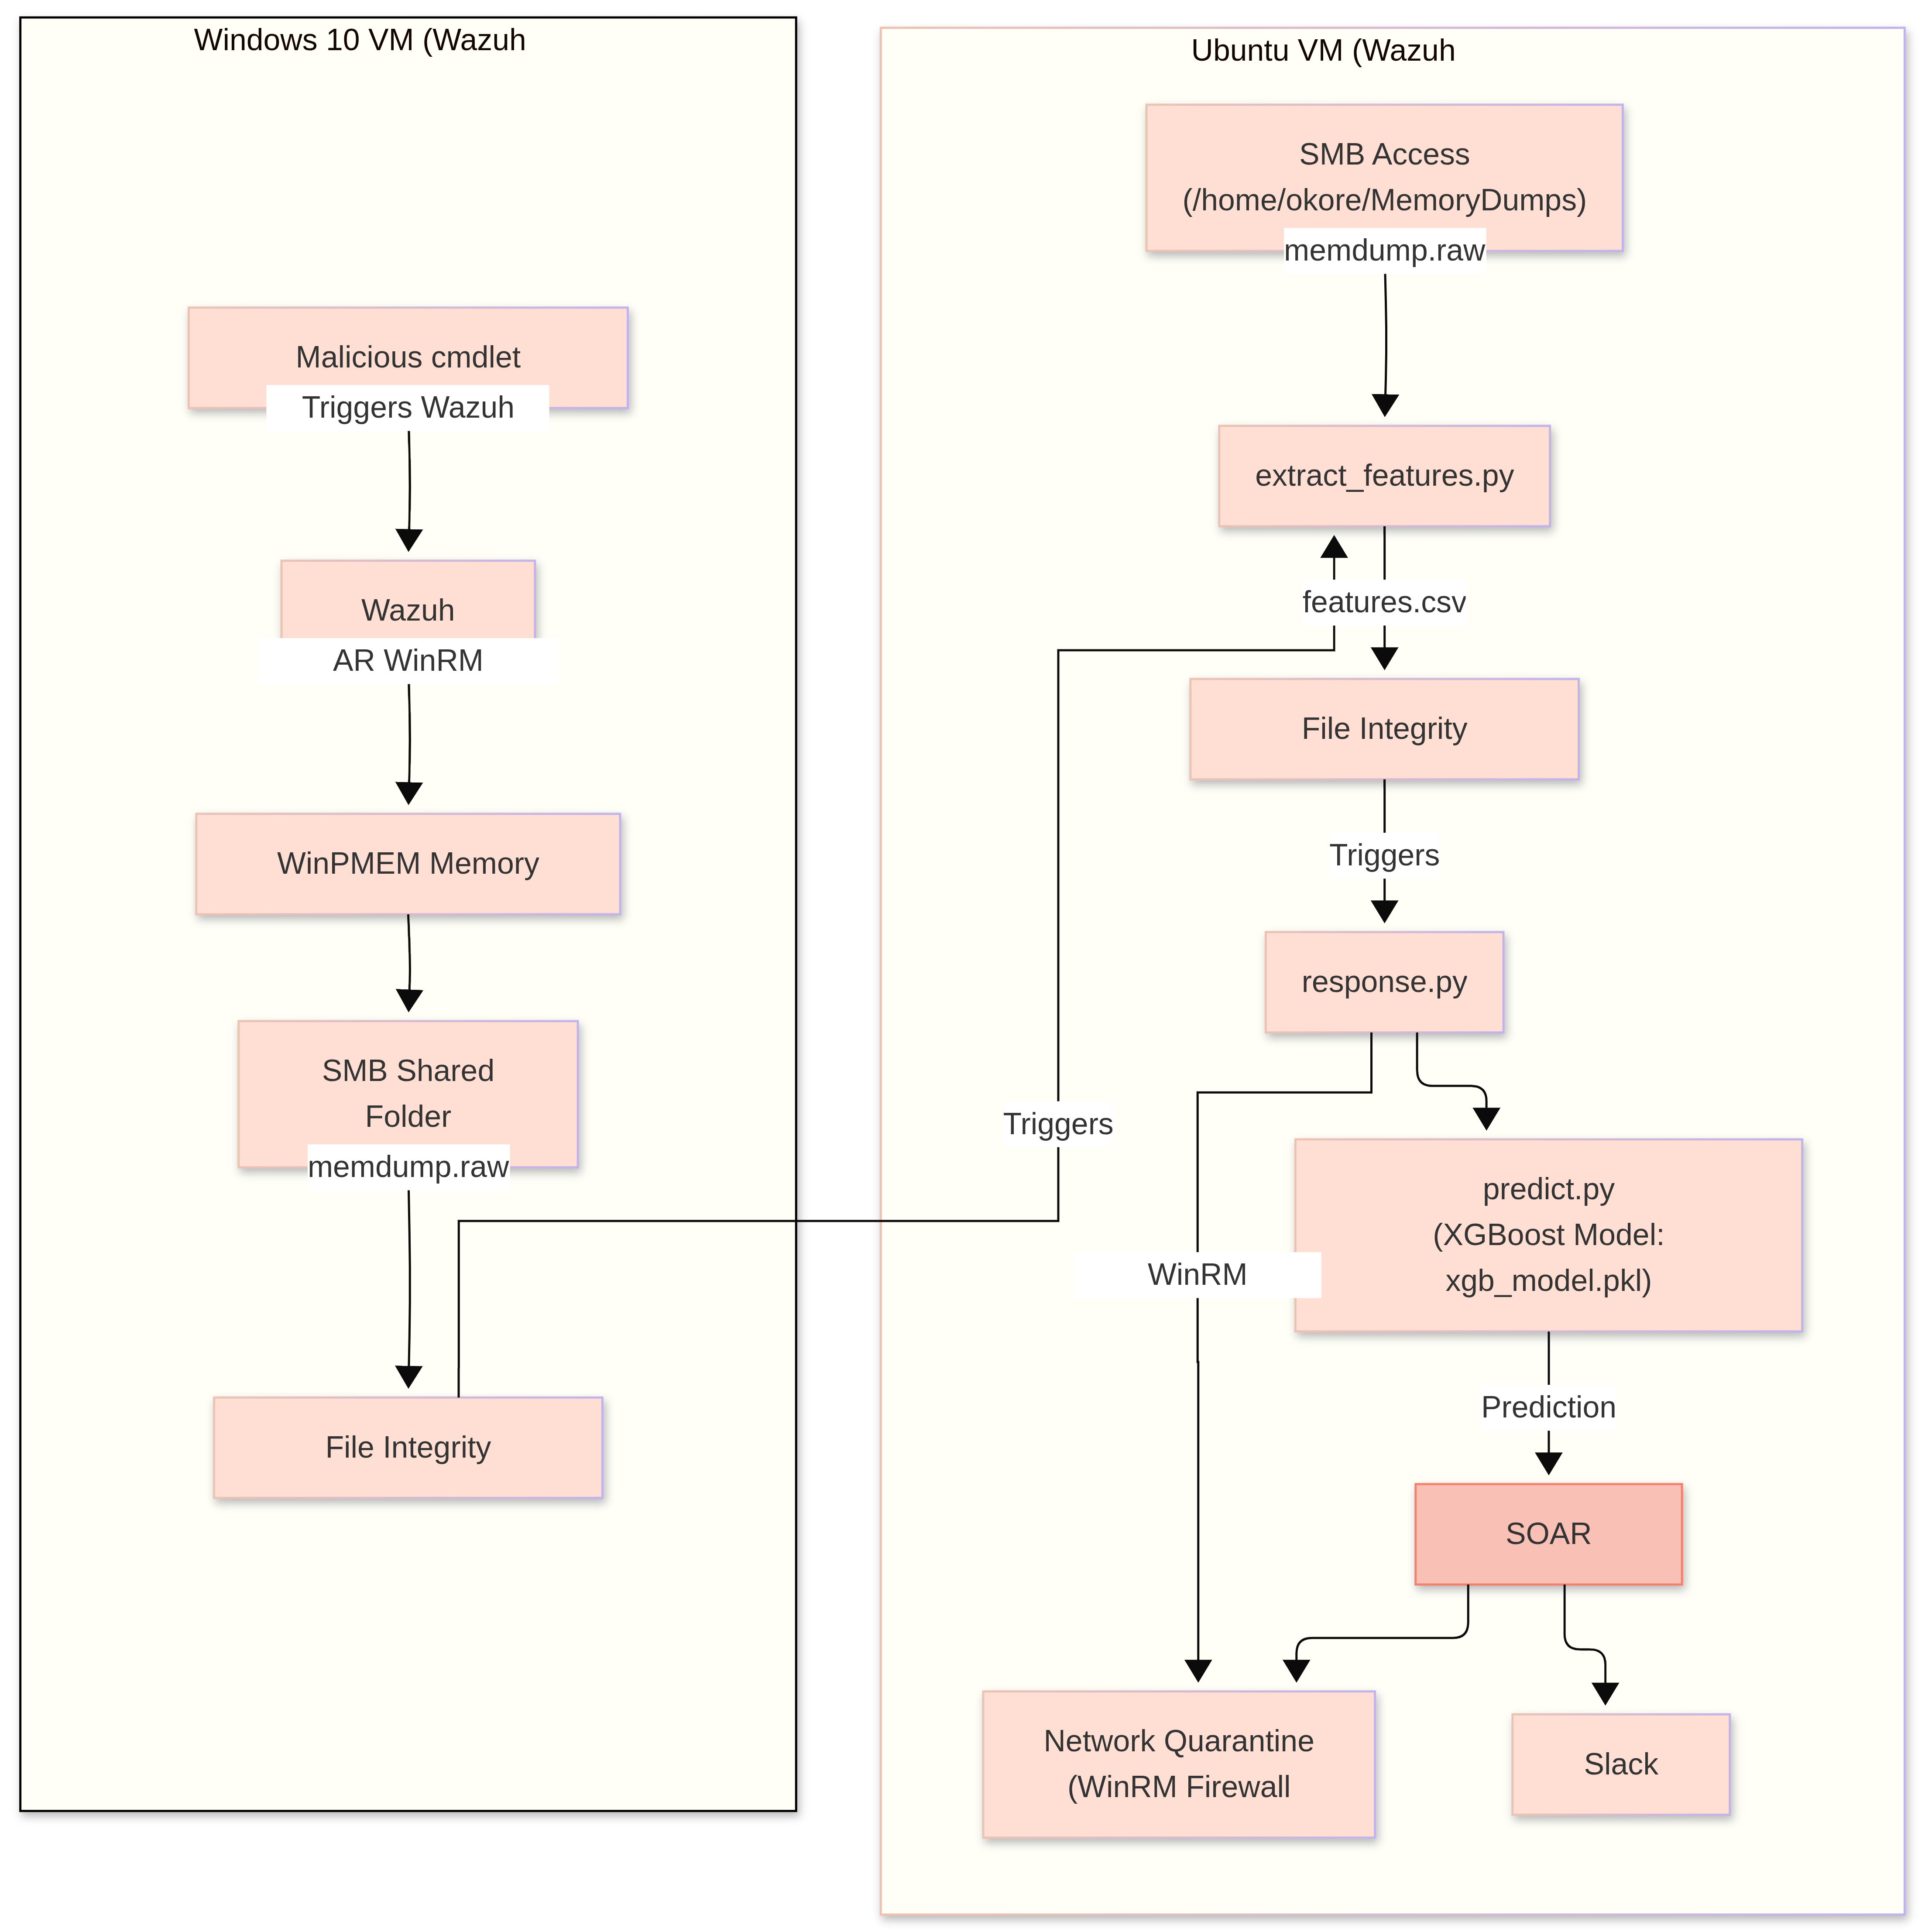
\includegraphics[width=\columnwidth]{SIBIRCON_arch_diag.png}
\caption{Deployment architecture and script-level workflow across the Windows
endpoint and Ubuntu manager.
% AR denotes Wazuh active response; SOAR denotes the automated response stage. Network quarantine is implemented by disabling endpoint network adapters over WinRM.
}
\label{fig:architecture}
\end{figure}

\subsection{Alert-Driven Memory Acquisition}
The Wazuh agent collects the Windows PowerShell operational log. Custom rules were configured to match indicators of compromise such as encoded-command execution and known offensive cmdlets. Wazuh active response scripts associated with these rules trigger memory dump acquisition on the monitored host and are configured with a severity level of 10. This stage uses the endpoint alert to trigger a memory dump of the monitored host, and subsequent classification is based on features extracted from the captured memory image.

The acquisition script reads the Wazuh JSON alert from standard input and extracts the agent name and IP address. It then invokes NetExec over WinRM to launch the preinstalled WinPMEM executable on that endpoint. The raw image is written to the configured dump path, and command output is appended to the acquisition log. Reading the target address from the alert connects the collection request to the endpoint that produced the triggering event.

This invocation is the only user-space process the pipeline's own code
starts on the endpoint prior to image acquisition: NetExec runs on the
manager and issues a single remote command, so the only endpoint-side
component involved before WinPMEM begins writing is the WinRM execution
host required to run that command, not an additional script of our own.
WinPMEM's acquisition is itself not passive: it loads a signed kernel
driver to obtain physical memory access, a precondition for live
acquisition on Windows that necessarily touches kernel memory state before
the image is written~\cite{winpmem}. The resulting image should therefore
be treated as a best-effort forensically sound capture of a running system,
consistent with the general limitation of live acquisition noted in the
digital-forensics literature, rather than a snapshot entirely unaffected by
the act of acquiring it.

The shared directory links the Windows acquisition path to the manager's analysis path. 
% Its use allows the analysis utilities to run on the manager while WinPMEM operates on the endpoint. 
The prototype uses fixed image and feature filenames suitable for a single-endpoint experiment. Concurrent incidents from different endpoints would require separate artifact locations and identifiers.

\subsection{Event-Driven Orchestration}
Wazuh File Integrity Monitoring (FIM) coordinates the pipeline by detecting changes to the memory image and feature CSV. Changes to the raw memory image trigger feature extraction through rules 100100/100101. Changes to the feature CSV invoke the response script through rules 100102/100103; this script classifies the extracted features and applies the response policy. These custom rules are defined specifically for the pipeline and are not included in Wazuh's default ruleset. Their identifiers were chosen arbitrarily, and the active-response configuration associates each rule with the corresponding pipeline script. The file-change events determine when each stage runs, while the files provide the data it processes. Table~\ref{tab:interfaces} summarizes the inputs and
outputs of each component.

\begin{table}[t]
\caption{Pipeline Components and Data Interfaces}
\label{tab:interfaces}
\centering
\footnotesize
\begin{tabular}{@{}p{1.45cm}p{2.85cm}p{3.55cm}@{}}
\toprule
Component & Input or trigger & Output or action \\
\midrule
Acquisition & Wazuh alert JSON & Remote WinPMEM invocation; raw memory image \\
Extraction & Image-file FIM event & Forensic feature vector in CSV format \\
Classifier & Feature vector & Class label and model score in JSON \\
Response & Feature-file FIM event and prediction & Network isolation request; analyst notification \\
\bottomrule
\end{tabular}
\end{table}

% The interfaces define three representations of an incident: the captured memory state, the trigger event, and the decision supplied to the response policy. Retaining these intermediate artifacts supports inspection of the relationship between evidence and action. It also permits changes to feature extraction or classification without redesigning acquisition, provided that the associated input and output interfaces remain compatible.

% The current implementation uses file modifications as transition events. This provides a direct integration with Wazuh FIM, but does not enforce file completion or unique event processing. The corresponding requirements for completion detection and duplicate suppression are addressed in Section~\ref{sec:discussion}.

The pipeline produces a memory image, a CSV file of extracted features, and a classification result. Together with the recorded Wazuh events, these artifacts allow an analyst to trace how captured evidence leads to a response decision. Defined file and message interfaces also allow the feature extractor or classifier to be updated without changing memory acquisition, provided that each component continues to accept the expected inputs and produce the outputs required by the next stage.

A file modification triggers the next stage, so a naive write-in-place would let feature extraction or classification begin before its input file is complete. Both the memory image and the feature CSV are instead published through a staging-then-atomic-rename sequence: each artifact is written to a path FIM does not watch, and only moved onto the watched path once writing has finished, so FIM observes only complete files at the acquisition and extraction stages. Repeated events for the same file may still invoke a stage more than once; Section~\ref{sec:discussion} discusses the duplicate-event
handling needed to address this remaining limitation.


\subsection{Forensic Feature Representation and Classification}
Classification uses two features derived from Volatility3 service-scan output: the number of service records, \texttt{svcscan.nservices}, and the number of distinct nonzero process identifiers associated with those records, \texttt{svcscan.process\_services}. This aggregation converts the plugin's variable-length output into a fixed-length representation of Windows service state and confines extraction to a single plugin.

The extractor publishes a feature record only when Volatility returns
nonempty service output. An unsuccessful plugin invocation or an empty result
is logged, and the script returns before writing a new CSV. This check
prevents an absent service scan from being represented as a valid vector of
zero-valued counters. It does not establish the completeness of the underlying
memory image or remove a feature file left by an earlier invocation.

An XGBoost model performs binary classification of the resulting vector. Preprocessing uses a standardization transform fitted on the training partition and serialized with the model. Inference applies the same transform and feature ordering. The original two-feature model achieved 99.84\% accuracy on a 70/30 split of the pre-processed CIC-MalMem-2022 dataset. This is a benchmark result on a public dataset, not a measurement of accuracy on deployment endpoints; Section~\ref{sec:assessment} examines what the result depends on and what would be required before using it for containment decisions.

The decision interface consists of a JSON message containing the numeric label, class name, and malicious-class model score. The predicted label controls the response policy; the score provides additional context in the analyst notification. The implementation initiates containment for label one and leaves the endpoint unchanged for a benign prediction. A JSON parsing failure terminates this invocation without a containment request.

\subsection{Response Policy and Operational Records}
The response policy combines endpoint containment with analyst notification. A malicious classification initiates a WinRM command that disables the endpoint's network adapters. Notification is handled on the Ubuntu manager, which sends the affected host, predicted class, and classification score to Slack after requesting isolation. This placement allows notification to proceed independently of the endpoint's network availability following containment.

WinRM credentials and the notification webhook are supplied through environment variables. Operational records cover acquisition, extraction, classification, and response, providing evidence of execution at each stage. The distinction between command execution and its effect is evaluated through both response logs and endpoint connectivity observations in Section~\ref{sec:case}.

Each stage also computes a SHA-256 digest of the artifact it produces, or
of the artifact it consumes before acting on it, and appends the digest to
a shared, append-only integrity log: the acquired image is hashed once it
is visible to the manager and again by the extraction script before
Volatility runs on it, the feature CSV is hashed immediately after it is
written, and the classification decision is hashed by both the classifier
and the response script that receives it. This produces a verifiable
chain from the specific byte sequence acquired on the endpoint, through
the features derived from it, to the decision that triggered containment,
so a later discrepancy between any two stages' recorded digests for the
same artifact is directly detectable rather than inferred.

Containment and notification have separate observable outcomes. The
notification client records whether Slack accepts the message, using the HTTP
response status, and logs delivery errors. Message delivery establishes that
the manager has reported its decision; it does not verify that the endpoint
has been isolated. Assessing the complete response therefore requires evidence
from both the remote action and the notification client.

\section{Experimental Evaluation}
\label{sec:case}

\subsection{Testbed and Evaluation Criteria}
The evaluation uses an isolated two-VM testbed comprising a Windows 10 endpoint and an Ubuntu Wazuh manager. PowerShell event collection and FIM supply the detection inputs; WinRM and an SMB share provide the control and artifact-access paths. In the evaluation scenario, WannaCry ransomware was introduced through a PowerShell download-and-execution sequence which triggered automated memory dump acquisition on the monitored endpoint.
% from a server within the testbed.

Functional evaluation considers three properties: automatic invocation of successive stages, propagation of the acquired evidence through classification, and execution of the configured response. Wazuh events and script outputs provide evidence of stage invocation and artifact processing. Response logs and a subsequent endpoint connectivity test assess the containment and notification behavior. Workflow latency is measured between subsequent stages of the pipeline.
% acquisition-script and response-script start times.
The experiment evaluates integration in one malware scenario; the scope of generalization is discussed in Section~\ref{sec:discussion}.

\subsection{Functional Integration and Response}
The WannaCry experiment demonstrates automatic progression through acquisition, feature extraction, classification, and response. Raw-image and feature-file FIM events correspond to the configured extraction and response rules, while successful Volatility3 dump analysis and artifact extraction establishes that the acquired image reached the analysis stage. The resulting feature vector produced a malicious classification and activated the containment policy.

Table~\ref{tab:observations} relates these results to the evaluation criteria. The response script's execution log records an isolation request and a successful Slack notification. In the endpoint connectivity test, all four outbound probes from the isolated endpoint failed with local transmission errors, confirming that the network adapters were disabled as a result of the isolation.
% These observations support the functional operation of the response path in the testbed, without establishing coverage of every possible communication path.

\begin{table}[t]
\caption{Functional Evaluation of the Integrated Pipeline}
\label{tab:observations}
\centering
\footnotesize
\begin{tabular}{@{}p{2.5cm}p{5.55cm}@{}}
\toprule
Evaluation criterion & Experimental evidence \\
\midrule
Automatic stage invocation & Acquisition trigger and image/feature FIM events activate the configured stages \\
Evidence processing & Successful service scan, feature extraction, and classification \\
Containment & Isolation request and four failed endpoint connectivity probes \\
Analyst notification & Successful Slack delivery reported by the response client \\
\bottomrule
\end{tabular}
\end{table}

The separation of the classifier from response policy makes the feature vector and predicted label available for inspection at the decision boundary.
% The current decision message uses JSON; the experiment's retained screenshot uses an earlier dictionary-style serialization of the decision fields. This format difference does not alter the label-based response policy.

\subsection{Workflow Latency}
The pipeline reached the response stage 171\,s (2\,min 51\,s) after the acquisition stage started. Table~\ref{tab:timing} reports the available timestamps for the start of each stage. The acquisition-to-extraction interval is 60\,s, followed by 111\,s between extraction and response initiation. These intervals include both stage processing and the associated orchestration overhead.

\begin{table}[t]
\caption{Stage-Start Timing in the WannaCry Experiment}
\label{tab:timing}
\centering
\small
\begin{tabular}{@{}lrr@{}}
\toprule
Stage & Start time & Elapsed from acquisition \\
\midrule
Acquisition & 23:44:09 & 0\,s \\
Feature extraction & 23:45:09 & 60\,s \\
Prediction and response & 23:47:00 & 171\,s \\
\bottomrule
\end{tabular}
\par\smallskip
\begin{minipage}{\columnwidth}\footnotesize
% Timestamps: 16 May 2025, MSK. Elapsed time is measured between stage starts.
\end{minipage}
\end{table}

The measured interval spans the start of memory acquisition to the start of the response stage.
% Initial malicious execution and completed containment lack separate timestamps, preventing a full detection-to-containment latency estimate.
The experiment demonstrates automated execution of the integrated workflow in the testbed. Repeated trials with different memory sizes, workloads, and numbers of concurrently processed endpoints are
needed to assess how response times vary across operating conditions.

More detailed timing would help identify where delays occur within the workflow. Recording the completion of image writing, receipt of each FIM event, completion of feature extraction, and the verification of endpoint isolation would separate processing time from the waiting periods between stages. These measurements would show whether a change in response time is associated with acquisition, event delivery, analysis, or containment. They would also support comparisons between sequential and concurrent endpoint processing under the same evaluation protocol.

\section{Classifier Assessment}
\label{sec:assessment}

\subsection{Benchmark Performance}
The deployed classifier uses two service features. To examine how much
classification performance depends on this representation, the supporting
evaluation compares it with larger feature sets from CIC-MalMem-2022.
The dataset contains 58{,}596 records, equally divided between benign and
malicious classes, and 55 numeric features~\cite{carrier2022,cicmalmem}.
Removing constant features leaves 52 predictors. For each feature set,
an XGBoost model is trained using 200 estimators and a maximum tree depth
of 6. All models use the same stratified 70/30 training/test split with
random seed 7, with standardization fitted only on the training data.

Accuracy on the test partition is 99.99\% with all 52 predictors, 99.98\%
with six host-configuration counters, and 99.84\% with the two service
features. For a descriptive comparison across the entire dataset, a rule
labels a record as malicious when its service count is 391 or lower, or
greater than 1000. This rule correctly classifies 99.63\% of all records.
The small differences between the model results indicate that a compact
set of host-state counters can reproduce much of the benchmark accuracy.

\subsection{Implications for Deployment}
Further checks examine the class distributions underlying these results.
Benign records have higher medians for all 22 selected count and count-derived
indicators. Using total handle count as a proxy for system load, a procedure
trims the data to an overlapping range and matches equal numbers of benign
and malicious records within handle-count ranges. It retains 148 records,
comprising 74 from each class.

A separate five-fold logistic-regression analysis using all 52 predictors
assigns a malicious-class probability between 0.1 and 0.9 to only 0.92\% of
records. Most predicted probabilities therefore lie near the benign or
malicious extreme. 
% These checks describe class separation in the dataset;they do not establish whether collection conditions caused it.
The reported use of SMOTE to generate synthetic records~\cite{carrier2022} also raises
the possibility of related samples appearing in both random partitions.
The available provenance is insufficient to confirm or quantify such dependence.
For the response system, the implication is to evaluate the classifier on
representative endpoint captures before using it for routine containment.

\subsection{Host-Relative Scoring}
A separate preliminary study examines whether memory features can be assessed relative
to clean captures from the same host. The implementation extracts 44 features
from eight Volatility3 plugins and measures each feature's departure from
its reference value. This baseline-differential scorer is evaluated
separately from the XGBoost containment path.

For feature $i$, let $m_i$ be its clean-reference median and $d_i$ its median
absolute deviation multiplied by 1.4826. For a capture $x$, the standardized
deviation and overall score are
\begin{equation}
z_i(x)=\frac{x_i-m_i}{s_i+10^{-9}},\qquad
S_F(x)=\max_{i\in F}|z_i(x)|,
\end{equation}
where $F$ is the selected feature set. The scale is $s_i=d_i$ unless
$d_i<10^{-6}$, in which case $s_i=\max(0.01|m_i|,1)$. This fallback handles
features with negligible variation in the reference captures. The score is
the largest absolute standardized deviation, so a high value indicates that
at least one feature differs substantially from its reference value relative
to the chosen scale.

The study consists of ten sequential pre/post pairs from one Windows Server
2022 VM, collected around Atomic Red Team~\cite{atomicredteam} tests for
MITRE ATT\&CK T1055.001, .002, .003, .004, and .012~\cite{mitre1055}.
Only the first six pairs are retained for scoring. Pre-test
\texttt{malfind.commitCharge} values rise from 259--265 in trials 1--6 to
773--778 in trials 7--10, showing that the later reference state has changed.
Incomplete cleanup is a plausible explanation, but the aggregate records
do not identify the responsible process.

Scoring compares all 44 features with a restricted set of 11
\texttt{malfind} and \texttt{ldrmodules} features. With the restricted set,
scores increase from 0.797 to 3.000 for the APC-injection pair and from
4.000 to 5.000 for the process-hollowing pair. None of the six retained
post-test captures reaches the default threshold of 6. Using all 44
features flags three post-test captures and one pre-test reference capture.
Because the six pre-test captures also fit the reference model, these
results do not provide an independent estimate of the false-positive rate.
The study therefore identifies requirements for representative reference
captures and independent threshold calibration before the scorer can be
used to control containment.

\section{Discussion}
\label{sec:discussion}

\subsection{Operational Value and Response Ordering}
The operational value of the system is that an endpoint alert can initiate forensic collection and carry the resulting evidence through to a response decision. The WannaCry case study demonstrates this progression without manual stage invocation. The acquired image, feature record, and classification output also support analyst review of the decision. Assessing the effect on analyst workload requires comparison with a manual workflow.

The order of these stages also affects how long a contaminated endpoint remains connected. The evaluated configuration collects and analyzes memory before isolation to preserve WinRM and SMB access. The contaminated endpoint therefore remains connected during this interval. The appropriate ordering depends on the incident policy and the availability of management paths that remain accessible after isolation.

The containment policy also needs a defined recovery procedure. Since the implemented action disables the network adapters used for WinRM, restoring connectivity requires a path that does not depend on that connection. A deployment procedure would need to specify how an analyst authorizes release and how connectivity is restored. These steps lie outside the scope of this study, as demonstrated in the memory forensic workflow.

\subsection{Reliability Requirements}
% Reliable analysis requires completed input files and protection against repeated invocation.
The acquisition and extraction stages now publish artifacts through atomic rename, as described in Section~\ref{sec:architecture}, which addresses premature triggering on a partially written file. Duplicate-event suppression for repeated FIM events on the same completed file remains unaddressed. Incident-specific artifact paths are also needed to keep concurrent captures separate.

Containment reliability depends on verifying the command's effect on the endpoint. The isolation wrapper now checks the remote command's exit status, logs a hash of its output, and reports failure rather than unconditionally declaring the endpoint isolated. This confirms that the remote command completed, but not independently that the network adapters are down; the connectivity probe used in the case study is still the only check of actual containment effect, and it is not yet invoked automatically as part of each response.

\subsection{Evaluation Scope and Further Validation}
These reliability requirements must be evaluated beyond the current demonstration. The system evaluation covers one Windows endpoint and one WannaCry experiment, establishing functional integration in that setting. It does not determine throughput under concurrent load, latency variability, recovery from failed stages, or detection coverage across malware families.

The supporting host-relative study informs baseline design but does not validate a replacement classifier. Workload and technique are coupled in a fixed rotation, and retained evidence lacks raw memory images and per-test execution transcripts. Broader validation should therefore combine repeated system trials under varied workloads, independent classifier calibration using representative endpoint captures, and tests of recovery after acquisition or response failures.


% Keep the conclusion together and balance the final-page columns.
% Revisit this column break after substantive changes to manuscript length.
\newpage
\section{Conclusion}

This work demonstrates the integration of memory forensics into an automated incident-response workflow. The implemented system uses Wazuh active-response rules to coordinate memory acquisition, forensic analysis, classification, and containment across a Windows endpoint and an Ubuntu manager. In the isolated WannaCry experiment, the pipeline executed without manual stage invocation and reached response initiation in under three minutes from the start of memory acquisition. Execution logs document the isolation request and analyst notification, while subsequent connectivity observations support the effect of the containment action.

The system's contribution is to connect forensic evidence collection directly to endpoint response while making the memory image, extracted features, and classification result available for analyst inspection. The supporting
classifier assessment highlights the need to validate decisions on captures representative of the deployment environment. Further development will strengthen evaluation of performance and failure recovery across multiple endpoints and workloads.
\begin{thebibliography}{10}
\bibitem{wazuh} Wazuh, ``Active Response,'' \textit{Wazuh Documentation}.
Accessed: Sep. 9, 2026. [Online]. Available:
\url{https://documentation.wazuh.com/current/user-manual/capabilities/active-response/index.html}

\bibitem{winpmem} Velocidex, ``WinPmem: A Physical Memory Acquisition Tool.''
Accessed: Sep. 9, 2026. [Online]. Available:
\url{https://github.com/Velocidex/WinPmem}

\bibitem{volatility} Volatility Foundation, ``Volatility 3 Documentation.''
Accessed: Sep. 9, 2026. [Online]. Available:
\url{https://volatility3.readthedocs.io/en/latest/}

\bibitem{cohen2011} M. I. Cohen, D. Bilby, and G. Caronni,
``Distributed forensics and incident response in the enterprise,''
\textit{Digital Investigation}, vol. 8, suppl., pp. S101--S110, 2011,
doi: \href{https://doi.org/10.1016/j.diin.2011.05.012}{10.1016/j.diin.2011.05.012}.

\bibitem{syed2026} A. T. Syed, M. C. Ghanem, E. Benkhalifa, and
F. A. Idrees, ``SPECTRE: a hybrid and adaptive cyber threats detection and
response in volatile memory,'' \textit{Int. J. Information Security},
vol. 25, Art. no. 52, 2026,
doi: \href{https://doi.org/10.1007/s10207-026-01212-6}{10.1007/s10207-026-01212-6}.

\bibitem{lashkari2021} A. H. Lashkari, B. Li, T. L. Carrier, and G. Kaur,
``VolMemLyzer: Volatile Memory Analyzer for Malware Classification using
Feature Engineering,'' in \textit{Proc. Reconciling Data Analytics,
Automation, Privacy, and Security: A Big Data Challenge (RDAAPS)},
2021, pp. 1--8,
doi: \href{https://doi.org/10.1109/RDAAPS48126.2021.9452028}{10.1109/RDAAPS48126.2021.9452028}.

\bibitem{carrier2022} T. Carrier, P. Victor, A. Tekeoglu, and A. H. Lashka1ri,
``Detecting Obfuscated Malware using Memory Feature Engineering,'' in
\textit{Proc. 8th Int. Conf. Information Systems Security and Privacy
(ICISSP)}, 2022, pp. 177--188,
doi: \href{https://doi.org/10.5220/0010908200003120}{10.5220/0010908200003120}.

\bibitem{okore2026} J. C. Okore, I. Womoakor, and I. V. Kotenko,
``Explainable Machine Learning for Effective Malware Detection in Encrypted
Network Traffic,'' in \textit{Proc. IEEE USBEREIT}, 2026, pp. 1--4,
doi: \href{https://doi.org/10.1109/USBEREIT70063.2026.11580625}{10.1109/USBEREIT70063.2026.11580625}.

\bibitem{arp2022} D. Arp, E. Quiring, F. Pendlebury, A. Warnecke,
F. Pierazzi, C. Wressnegger, L. Cavallaro, and K. Rieck,
``Dos and Don'ts of Machine Learning in Computer Security,'' in
\textit{Proc. 31st USENIX Security Symp.}, 2022, pp. 3971--3988.
[Online]. Available:
\url{https://www.usenix.org/conference/usenixsecurity22/presentation/arp}

\bibitem{projectrepo} J. C. Okore, ``CCF-Project,'' GitHub repository.
[Online]. Available:
\url{https://github.com/Joellots/CCF-project}

\bibitem{cicmalmem} Canadian Institute for Cybersecurity,
``Malware Memory Analysis (CIC-MalMem-2022),'' University of New Brunswick.
Accessed: Sep. 9, 2026. [Online]. Available:
\url{https://www.unb.ca/cic/datasets/malmem-2022.html}

\bibitem{atomicredteam} Red Canary, ``Atomic Red Team.''
Accessed: Sep. 9, 2026. [Online]. Available:
\url{https://github.com/redcanaryco/atomic-red-team}

\bibitem{mitre1055} MITRE, ``Process Injection, Technique T1055,''
\textit{MITRE ATT\&CK}.
Accessed: Sep. 9, 2026. [Online]. Available:
\url{https://attack.mitre.org/techniques/T1055/}

\end{thebibliography}
\end{document}
